\documentclass[aspectratio=169]{beamer}
\usetheme[block=fill]{metropolis}
\usepackage{tikz}
\usetikzlibrary{shapes.geometric, arrows.meta, positioning, calc}

\title{Building a Reproducible Scholarly Search Toolkit}
\subtitle{Episode 23: The Importer Subsystem (Reading RIS)}
\author{Scholar Search Kit}
\date{}

\begin{document}

\begin{frame}[plain]
  \titlepage
\end{frame}

\begin{frame}{Episode Goal}
  \begin{alertblock}{The Goal}
    Create the \texttt{RISImporter} to read standard academic exports from external databases like Scopus or Web of Science.
  \end{alertblock}
  \vspace{0.5cm}
  Sometimes the best data source doesn't have an API. Researchers will manually export a \texttt{.ris} file from their university library. Our tool must be able to absorb it.
\end{frame}

\begin{frame}{The Pipeline Reversal}
  \begin{center}
  \resizebox{0.6\linewidth}{!}{
  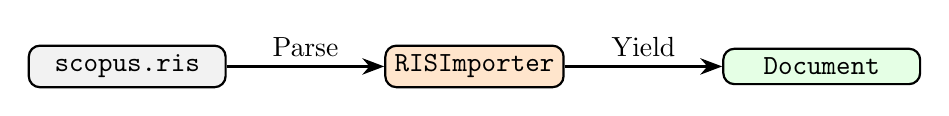
\begin{tikzpicture}[
      node distance=1cm and 2cm,
      file/.style={rectangle, draw, thick, rounded corners, minimum width=2.5cm, align=center, fill=black!5},
      imp/.style={rectangle, draw, thick, rounded corners, minimum width=2cm, align=center, fill=orange!20},
      model/.style={rectangle, draw, thick, rounded corners, minimum width=2.5cm, align=center, fill=green!10},
      arrow/.style={-{Stealth[scale=1.2]}, thick}
    ]
    
    \node[file] (f) {\texttt{scopus.ris}};
    \node[imp, right=of f] (im) {\texttt{RISImporter}};
    \node[model, right=of im] (d) {\texttt{Document}};
    
    \draw[arrow] (f) -- node[above] {Parse} (im);
    \draw[arrow] (im) -- node[above] {Yield} (d);
  \end{tikzpicture}
  }
  \end{center}
  \vspace{0.2cm}
  This is the exact inverse of our \texttt{RISExporter} from Episode 16.
\end{frame}

\begin{frame}{Implementation: Parsing the Loop}
  \begin{block}{Stateful Iteration}
    RIS files separate records using the \texttt{ER  -} tag.
  \end{block}
  
  \begin{itemize}
      \item We read the file line by line to keep memory footprint at O(1).
      \item We build a temporary dictionary of tags (\texttt{TI} for title, \texttt{DO} for DOI).
      \item When we hit \texttt{ER  -}, we instantiate a \texttt{Document} and \texttt{yield} it.
  \end{itemize}
\end{frame}

\begin{frame}{Verification}
  \begin{alertblock}{Success Criteria}
    \begin{itemize}
        \item The \texttt{RISImporter} can read a 10,000 line RIS file instantly without crashing.
        \item The yielded \texttt{Document} models have correctly populated `ExternalIds`.
    \end{itemize}
  \end{alertblock}
\end{frame}

\end{document}
